\documentclass[$if(fontsize)$$fontsize$,$endif$$if(lang)$$babel-lang$,$endif$$if(papersize)$$papersize$paper,$endif$$for(classoption)$$classoption$$sep$,$endfor$]{$documentclass$}

$for(bibliography)$
\addbibresource{$bibliography$}
$endfor$

\providecommand{\tightlist}{%
    \setlength{\itemsep}{0pt}\setlength{\parskip}{0pt}}

\begin{document}

$if(title)$
\title{$title$}
$endif$
$if(author)$
\author{$author$}
$endif$
$if(advisor)$
\advisor{$advisor$}
$endif$
$if(coadvisor)$
\coadvisor{$coadvisor$}
$endif$
$if(defenddate)$
\defenddate{$defenddate$}
$endif$
$if(school)$
\school{$school$}
$endif$
$if(institute)$
\institute{$institute$}
$endif$
$if(studentnumber)$
\studentnumber{$studentnumber$}
$endif$
$if(major)$
\major{$major$}
$endif$

$if(englishtitle)$
\englishtitle{$englishtitle$}
$endif$
$if(englishauthor)$
\englishauthor{\textsc{$englishauthor$}}
$endif$
$if(englishadvisor)$
\englishadvisor{Prof. \textsc{$englishadvisor$}}
$endif$
$if(englishcoadvisor)$
\englishcoadvisor{Prof. \textsc{$englishcoadvisor$}}
$endif$
$if(englishschool)$
\englishschool{$englishschool$}
$endif$
$if(englishinstitute)$
\englishinstitute{\textsc{$englishinstitute$} \\
  \textsc{Shanghai Jiao Tong University} \\
  \textsc{Shanghai, P.R.China}}
$endif$
$if(englishmajor)$
\englishmajor{$englishmajor$}
$endif$
$if(englishdate)$
\englishdate{$englishdate$}
$endif$
\maketitle

\makeatletter
\ifsjtu@submit\relax
	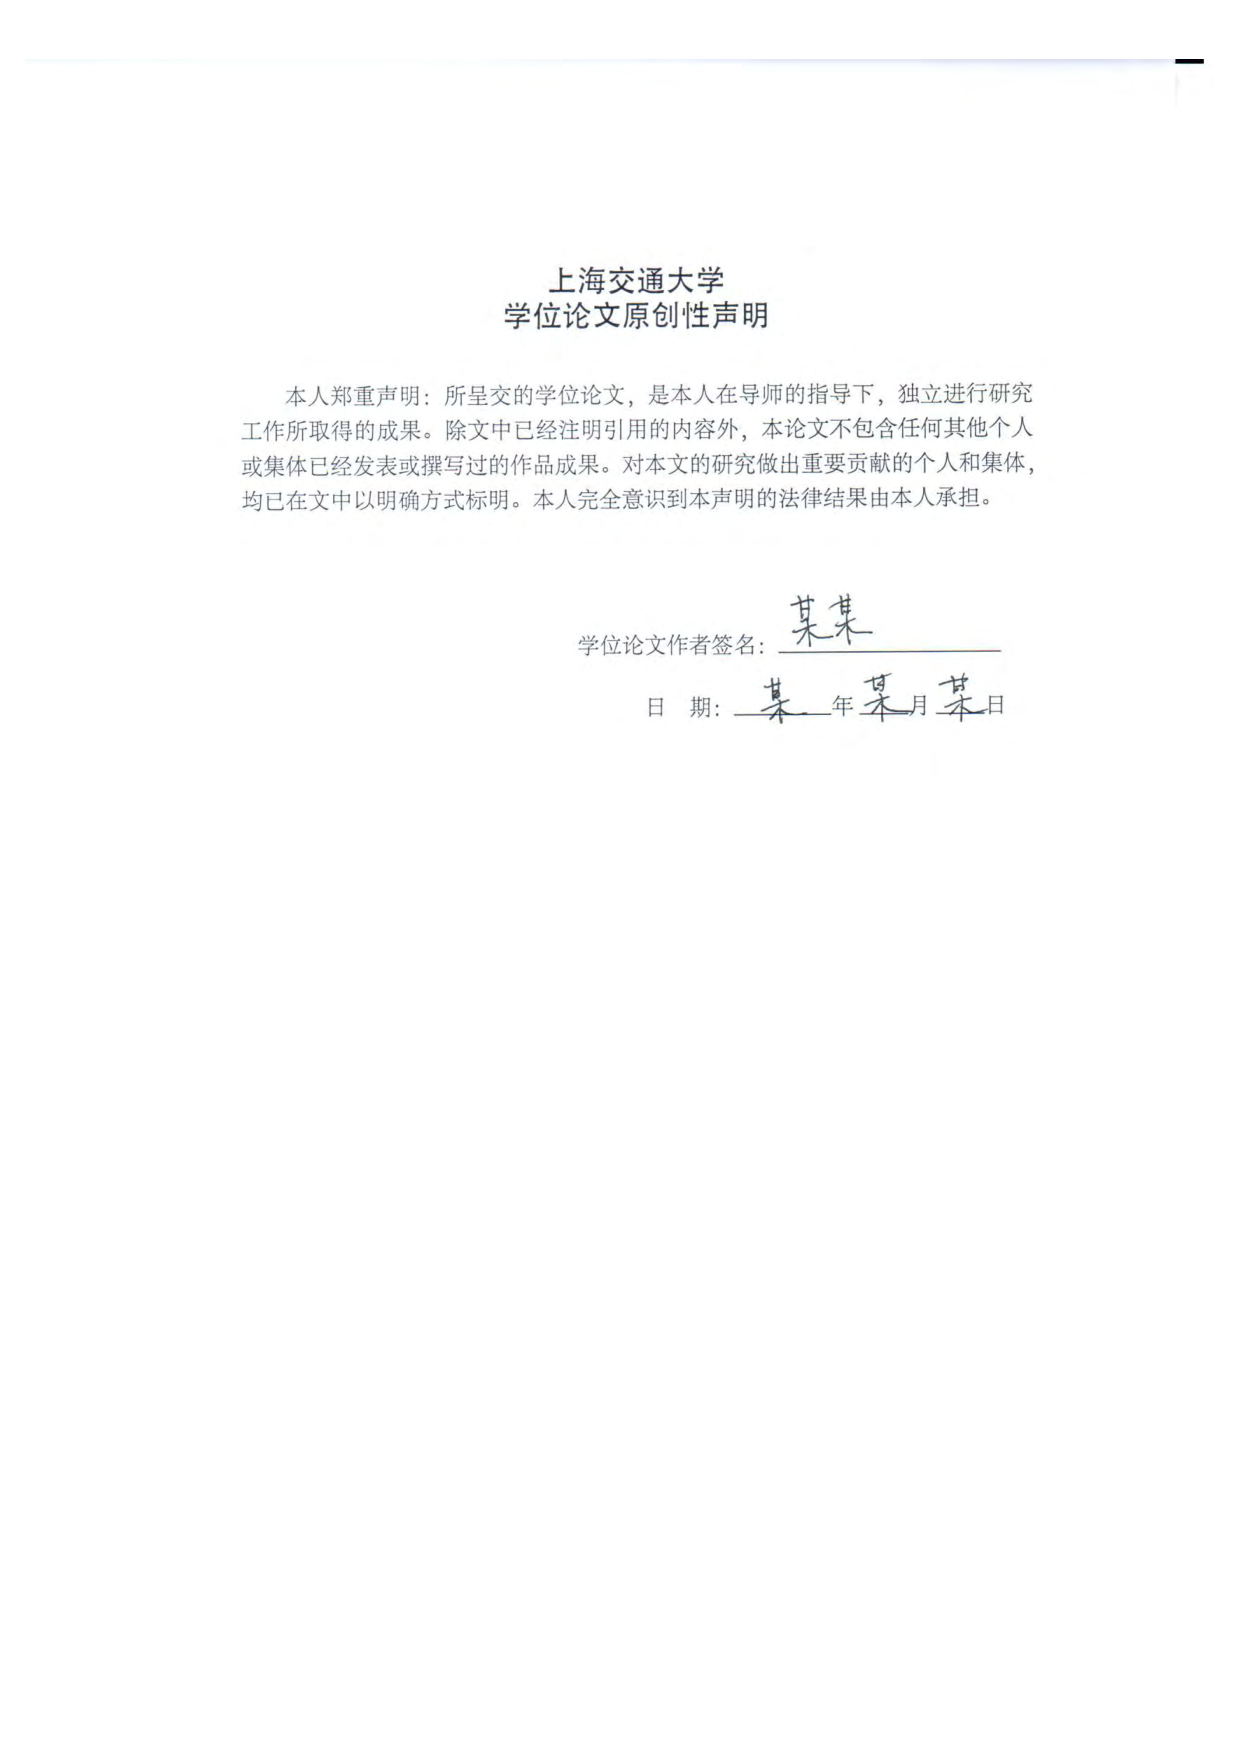
\includepdf{handed_pdf/original.pdf}
	\cleardoublepage
	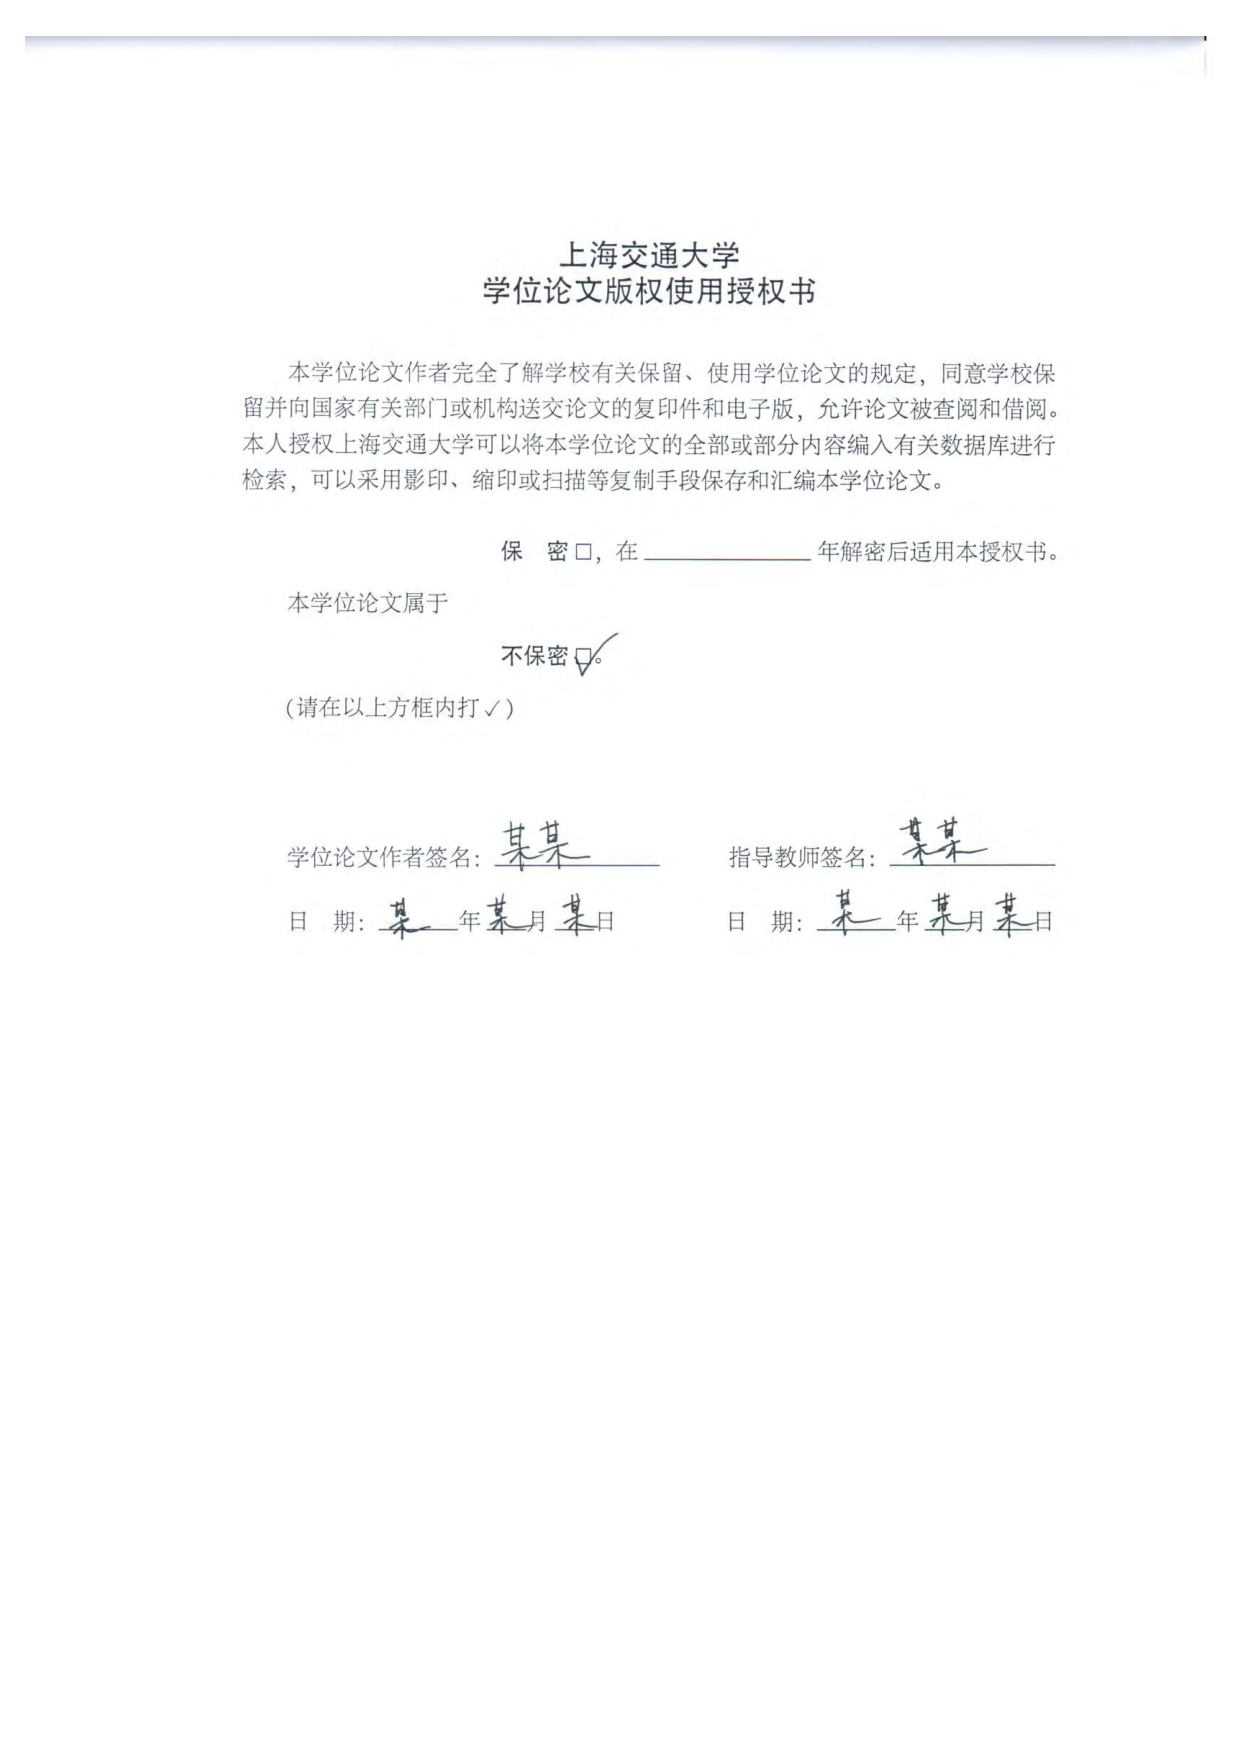
\includepdf{handed_pdf/authorization.pdf}
	\cleardoublepage
\else
\ifsjtu@review\relax
% exclude the original claim and authorization
\else
	\makeDeclareOriginal
	\makeDeclareAuthorization
\fi
\fi
\makeatother

$body$

\backmatter	% 文后无编号部分 

%% 参考资料
\printbibliography[heading=bibintoc]

%% 致谢、发表论文、申请专利、参与项目、简历
%% 用于盲审的论文需隐去致谢、发表论文、申请专利、参与的项目
\makeatletter

%%
% "研究生学位论文送盲审印刷格式的统一要求"
% http://www.gs.sjtu.edu.cn/inform/3/2015/20151120_123928_738.htm

% 盲审删去删去致谢页
\ifsjtu@review\relax\else
  %# -*- coding: utf-8-unix -*-
% !TEX program = xelatex
% !TEX root = ../thesis.tex
% !TEX encoding = UTF-8 Unicode
\begin{thanks}

  感谢所有测试和使用交大学位论文 \LaTeX 模板的同学!

  感谢那位最先制作出博士学位论文 \LaTeX 模板的交大物理系同学!

  感谢William Wang同学对模板移植做出的巨大贡献!
  
  感谢 \href{https://github.com/weijianwen}{@weijianwen} 学长一直以来的开发和维护工作!
  
  感谢 \href{https://github.com/sjtug}{@sjtug} 以及 \href{https://github.com/dyweb}{@dyweb} 对 0.9.5 之后版本的开发和维护工作!
  
  感谢所有为模板贡献过代码的同学们, 以及所有测试和使用模板的各位同学!

\end{thanks}
 	  %% 致谢
\fi

\ifsjtu@bachelor
  % 学士学位论文要求在最后有一个英文大摘要,单独编页码
  \pagestyle{biglast}
  % !TEX root = ../thesis.tex

\begin{bigabstract}
  An imperial edict issued in 1896 by Emperor Guangxu, established Nanyang
  Public School in Shanghai. The normal school, school of foreign studies,
  middle school and a high school were established. Sheng Xuanhuai, the person
  responsible for proposing the idea to the emperor, became the first president
  and is regarded as the founder of the university.

  During the 1930s, the university gained a reputation of nurturing top
  engineers. After the foundation of People's Republic, some faculties were
  transferred to other universities. A significant amount of its faculty were
  sent in 1956, by the national government, to Xi'an to help build up Xi'an Jiao
  Tong University in western China. Afterwards, the school was officially
  renamed Shanghai Jiao Tong University.

  Since the reform and opening up policy in China, SJTU has taken the lead in
  management reform of institutions for higher education, regaining its vigor
  and vitality with an unprecedented momentum of growth. SJTU includes five
  beautiful campuses, Xuhui, Minhang, Luwan Qibao, and Fahua, taking up an area
  of about 3,225,833 m2. A number of disciplines have been advancing towards the
  top echelon internationally, and a batch of burgeoning branches of learning
  have taken an important position domestically.

  Today SJTU has 31 schools (departments), 63 undergraduate programs, 250
  masters-degree programs, 203 Ph.D. programs, 28 post-doctorate programs, and
  11 state key laboratories and national engineering research centers.

  SJTU boasts a large number of famous scientists and professors, including 35
  academics of the Academy of Sciences and Academy of Engineering, 95 accredited
  professors and chair professors of the "Cheung Kong Scholars Program" and more
  than 2,000 professors and associate professors.

  Its total enrollment of students amounts to 35,929, of which 1,564 are
  international students. There are 16,802 undergraduates, and 17,563 masters
  and Ph.D. candidates. After more than a century of operation, Jiao Tong
  University has inherited the old tradition of "high starting points, solid
  foundation, strict requirements and extensive practice." Students from SJTU
  have won top prizes in various competitions, including ACM International
  Collegiate Programming Contest, International Mathematical Contest in Modeling
  and Electronics Design Contests. Famous alumni include Jiang Zemin, Lu Dingyi,
  Ding Guangen, Wang Daohan, Qian Xuesen, Wu Wenjun, Zou Taofen, Mao Yisheng,
  Cai Er, Huang Yanpei, Shao Lizi, Wang An and many more. More than 200 of the
  academics of the Chinese Academy of Sciences and Chinese Academy of
  Engineering are alumni of Jiao Tong University.
\end{bigabstract}

\else
  % 盲审论文中,发表学术论文及参与科研情况等仅以第几作者注明即可,不要出现作者或他人姓名
  \ifsjtu@review\relax
    %# -*- coding: utf-8-unix -*-
% !TEX program = xelatex
% !TEX root = ../thesis.tex
% !TEX encoding = UTF-8 Unicode

\begin{publications}{99}
    \item\textsc{第一作者}. {中文核心期刊论文}, 2007.  
    \item\textsc{第一作者}. {EI国际会议论文}, 2006.
\end{publications}

    %# -*- coding: utf-8-unix -*-
% !TEX program = xelatex
% !TEX root = ../thesis.tex
% !TEX encoding = UTF-8 Unicode

\begin{projects}{99}
    \item 参与973项目子课题(2007年6月--2008年5月)
    \item 参与自然基金项目(2005年5月--2005年8月)
    \item 参与国防项目(2005年8月--2005年10月)
\end{projects}
  
  \else
    %# -*- coding: utf-8-unix -*-
% !TEX program = xelatex
% !TEX root = ../thesis.tex
% !TEX encoding = UTF-8 Unicode
%%==================================================
%% pub.tex for SJTUThesis
%% Encoding: UTF-8
%%==================================================

\begin{publications}[99]
    \item\textsc{Chen H, Chan C~T}. {Acoustic cloaking in three dimensions using acoustic metamaterials}[J]. Applied Physics Letters, 2007, 91:183518.
    \item\textsc{Chen H, Wu B~I, Zhang B}, et al. {Electromagnetic Wave Interactions with a Metamaterial Cloak}[J]. Physical Review Letters, 2007, 99(6):63903.
\end{publications}
	      %% 发表论文
    % !TEX root = ../thesis.tex

%TC:ignore

\begin{projects}
  \item 参与973项目子课题(2007年6月--2008年5月)
  \item 参与自然基金项目(2005年5月--2005年8月)
  \item 参与国防项目(2005年8月--2005年10月)
\end{projects}

\begin{projects*}
  \item 973项目“XXX”
  \item 自然基金项目“XXX”
  \item 国防项目“XXX”
\end{projects*}

%TC:endignore
  %% 参与的项目
  \fi
\fi

% % !TEX root = ../thesis.tex

%TC:ignore

\begin{patents}
  \item 第一发明人,“永动机”,专利申请号202510149890.0
\end{patents}

\begin{patents*}
  \item 第一发明人,“永动机”,专利申请号XXXXXXXXXXXX.X
\end{patents*}

%TC:endignore
	  %% 申请专利
% % !TEX root = ../thesis.tex

%TC:ignore

\begin{resume}
  \subsection*{基本情况}
    某某,yyyy 年 mm 月生于 xxxx。

  \subsection*{教育背景}
  \begin{itemize}
    \item yyyy 年 mm 月至今,上海交通大学,博士研究生,xx 专业
    \item yyyy 年 mm 月至 yyyy 年 mm 月,上海交通大学,硕士研究生,xx 专业
    \item yyyy 年 mm 月至 yyyy 年 mm 月,上海交通大学,本科,xx 专业
  \end{itemize}

  \subsection*{研究兴趣}
    \LaTeX{} 排版

  \subsection*{联系方式}
  \begin{itemize}
    \item 地址: 上海市闵行区东川路 800 号,200240
    \item E-mail: \email{xxx@sjtu.edu.cn}
  \end{itemize}
\end{resume}

%TC:endignore
	  %% 个人简历

\makeatother

\end{document}
